% \iffalse
\let\negmedspace\undefined
\let\negthickspace\undefined
\documentclass[journal,12pt,twocolumn]{IEEEtran}
\usepackage{cite}
\usepackage{amsmath,amssymb,amsfonts,amsthm}
\usepackage{algorithmic}
\usepackage{graphicx}
\usepackage{textcomp}
\usepackage{xcolor}
\usepackage{txfonts}
\usepackage{listings}
\usepackage{enumitem}
\usepackage{mathtools}
\usepackage{gensymb}
\usepackage{comment}
\usepackage[breaklinks=true]{hyperref}
\usepackage{tkz-euclide} 
\usepackage{listings}
\usepackage{gvv}                                        
\def\inputGnumericTable{}                                
\usepackage[latin1]{inputenc}                            
\usepackage{color}                                       
\usepackage{array}                                       
\usepackage{longtable}                                   
\usepackage{calc}                              
\usepackage{tikz}
\usepackage{multirow}                                    
\usepackage{hhline}                                      
\usepackage{ifthen}                            
\usepackage{caption}
\usepackage{lscape}
\usepackage{amsmath}
\newtheorem{theorem}{Theorem}[section]
\newtheorem{problem}{Problem}
\newtheorem{proposition}{Proposition}[section]
\newtheorem{lemma}{Lemma}[section]
\newtheorem{corollary}[theorem]{Corollary}
\newtheorem{example}{Example}[section]
\newtheorem{definition}[problem]{Definition}
\newcommand{\BEQA}{\begin{eqnarray}}
\newcommand{\EEQA}{\end{eqnarray}}
\newcommand{\define}{\stackrel{\triangle}{=}}
\theoremstyle{remark}
\newtheorem{rem}{Remark}

\begin{document}

\bibliographystyle{IEEEtran}
\vspace{3cm}

\title{NCERT Math 11.9.2 Q8}
\author{EE23BTECH11009 - AROSHISH PRADHAN$^{*}$% <-this % stops a space
}
\maketitle
\newpage
\bigskip
\textbf{Question:} If the sum of $n$ terms of an AP is $(pn + qn^2)$, where $p$ and $q$ are constants, find the common difference.

\solution
\begin{table}[!h]
    \centering
    \begin{table}[!h]
    \centering
    \begin{tabular}{|c|c|c|}
    \hline
       \textbf{Symbol}  & \textbf{Value} &  \textbf{Description}\\
    \hline
       $V_{in}$  &  &  Input Voltage\\
    \hline
        $V_{out}$ & & Output Voltage\\
    \hline
        $f$ & $1000Hz$ & Input Wave Frequency\\
    \hline
        $T$ & $\dfrac{1}{f} = 10^{-3} s$ & Input Wave Time Period\\
    \hline
        \multirow{4}{*}{$R$} & (a) $0.5k\Omega$ & \multirow{4}{*}{Resistance}\\
        \cline{2-2}
        & (b) $5k\Omega$ &\\
        \cline{2-2}
        & (c) $0.5k\Omega$ &\\
        \cline{2-2}
        & (d) $5k\Omega$ &\\
    \hline
        \multirow{4}{*}{$C$} & (a) $0.1\mu F$ & \multirow{4}{*}{Capacitance}\\
        \cline{2-2}
        & (b) $1\mu F$ &\\
        \cline{2-2}
        & (c) $0.1\mu F$ &\\
        \cline{2-2}
        & (d) $1\mu F$ &\\
    \hline
        $\tau$ & $RC$ & Time Constant\\
    \hline
    \end{tabular}
    \caption{Given Parameters}
    \label{tab:1_gate.23.ph.37}
\end{table}

    \caption{Given Parameters}
    \label{tab:1}
\end{table}

Sum of $n$ terms, as a discrete signal:
\begin{align}
    s(n) = (pn + qn^2)u(n) \label{eq:1}
\end{align}
Taking the $Z$-Transform,
\begin{enumerate}
    \item $\mathcal{Z}\{nu(n)\}$

Using GP summation, 
\begin{align}
    \sum_{n = 0}^{\infty} z^{-n} &= \frac{1}{1 - z^{-1}}\\
    nu(n) &\system{Z} -zU'(z)\label{eq:3} \\ 
    \implies \sum_{n = 0}^{\infty} nz^{-n} &= \frac{z^{-1}}{(1-z^{-1})^2}\, \{\abs{z} > 1\} \label{eq:4}
\end{align}
\item $\mathcal{Z}{\{n^2 u(n)\}}$

From \eqref{eq:3},
    \begin{align}
        % \frac{d}{dz}\brak{\sum_{n = 0}^{\infty} nz^{-n}} &= \frac{d}{dz}\brak{ \frac{z^{-1}}{(1-z^{-1})^2}}\\
        % \implies \sum_{n = 0}^{\infty} -n^2 z^{-n-1} &= \frac{-z^{-2}(1+z^{-1})}{(1-z^{-1})^3}\\
        n^2 u(n) &\system{Z} -z\brak{\mathcal{Z}\{nu(n)\}}'\\
        \implies \sum_{n = 0}^{\infty} n^2 z^{-n} &= \frac{z^{-1}(1+z^{-1})}{(1-z^{-1})^3}\, \{\abs{z} > 1\} \label{eq:6}
    \end{align}
\end{enumerate}
Taking the Z-Transform of \eqref{eq:1} using \eqref{eq:4} and \eqref{eq:6}
\begin{align}
      S(z) = p\brak{\frac{z^{-1}}{(1-z^{-1})^2}} + q\brak{\frac{z^{-1}(1 + z^{-1})}{(1-z^{-1})^3}}
\end{align}
Now, 
\begin{align}
    s(n) &= x(n) \ast u(n)\\
    \implies S(z) &= X(z)U(z)\\
    \implies X(z) &= \frac{S(z)}{U(z)}\label{eq:12}
\end{align}
where,
\begin{align}
    U(z) &= \frac{1}{1 - z^{-1}}\label{eq:13}
\end{align}
Using \eqref{eq:13} in \eqref{eq:12},
\begin{align}
    X(z) &= p\brak{\frac{z^{-1}}{(1-z^{-1})}} + q\brak{\frac{z^{-1}(1 + z^{-1})}{(1-z^{-1})^2}}
\end{align}
Simplifying using partial fractions, we get:
\begin{align}
    X(z) &= (q-p) + \frac{p-3q}{1-z^{-1}} + \frac{2q}{(1-z^{-1})^2}\\
    &= (q - p) + \frac{(p-q)}{1-z^{-1}} + \frac{2qz^{-1}}{(1-z^{-1})^2}
\end{align}
Taking the inverse Z-Transform,
\begin{align}
    x(n) = (q-p)\delta(n) + (p-q)u(n) + 2qnu(n)\label{eq:15}
\end{align}
To simplify, use first term:
\begin{align}
    s(1) &= x(0)\\
    \implies p + q &= (q-p)\delta(0) + (p-q)u(0) + 2qnu(0)\\
    \implies p &= -q
\end{align}
because $\delta(0) = 1$ and $u(0) = 1$

$\therefore$ rewriting \eqref{eq:15}:
\begin{align}
    x(n) = 2q((n-1)u(n) + \delta(n))
\end{align}
Common difference is given by:
\begin{align}
    d &= x(n+1) - x(n)\\
    &= 2q(nu(n+1) + \delta(n+1)) - 2q((n-1)u(n) + \delta(n))\\
    &= 2q
\end{align}
\begin{figure}[!h]
    \centering
    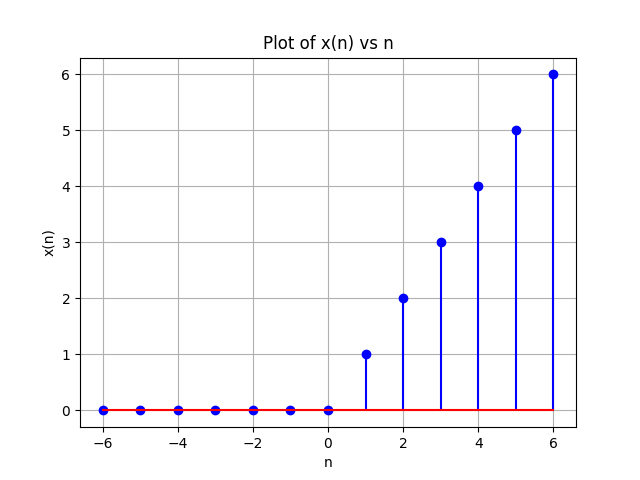
\includegraphics[width = \columnwidth]{figs/x_plot.png}
    \caption{Plot of x(n) vs n for $q=0.5$}
    \label{fig:1}
\end{figure}
\end{document}
